% \documentclass[handout]{beamer}
\documentclass{beamer}
\usepackage[ruled,linesnumbered]{algorithm2e}

\usepackage{natbib}
\definecolor{vuborange}{rgb}{1.0,0.40,0.0}
\usetheme{Boadilla}
\title{Step-wise Explanations of Constraint Satisfaction Problems}
\author{ Bart Bogaerts\textsuperscript{2}  \hspace{0.5cm}\underline{Emilio Gamba}\textsuperscript{1} \hspace{0.5cm} Tias Guns\textsuperscript{1}}
\date{}

\newcommand\m[1]{\ensuremath{#1}\xspace}
\newcommand\allconstraints{\m{T_P}}

\newcommand{\phantomgraphics}[2][]{%
  \leavevmode\phantom{\includegraphics[#1]{#2}}%
}


\makeatletter
\setbeamertemplate{footline}
{
  \leavevmode%
  \hbox{%
  \begin{beamercolorbox}[wd=.25\paperwidth,ht=2.25ex,dp=1ex,center]{author in head/foot}%
    \usebeamerfont{author in head/foot}E. Gamba (VUB, Brussels)
  \end{beamercolorbox}%
  \begin{beamercolorbox}[wd=.5\paperwidth,ht=2.25ex,dp=1ex,center]{title in head/foot}%
    \usebeamerfont{title in head/foot}Step-wise Explanations of Constraint Satisfaction Problems
  \end{beamercolorbox}%
  \begin{beamercolorbox}[wd=.25\paperwidth,ht=2.25ex,dp=1ex,right]{date in head/foot}%
    \usebeamerfont{date in head/foot}September 2020 \hspace*{2em}
    \insertframenumber{} / \inserttotalframenumber\hspace*{2ex} 
  \end{beamercolorbox}}%
  \vskip0pt%
}
\makeatother


\begin{document}

\begin{frame}
    \maketitle
    \vspace{-2.5cm}
    \begin{center}
        {\small\textsuperscript{1}Data Analytics Laboratory, Vrije Universiteit Brussel, Belgium\\
            \textsuperscript{2}Artificial Intelligence Lab, Vrije Universiteit Brussel, Belgium}
    \end{center}

    \begin{minipage}[t]{0.48\linewidth}
        \centering
        \vspace{0.1cm}
        \begin{figure}[h]
            
\includegraphics[width=\textwidth]{VUB-AI_RGB-1-800x223.png}
            \label{vub-logo}
        \end{figure}
    \end{minipage}\hfill
    \begin{minipage}[t]{0.48\linewidth}
        \centering
        \begin{figure}[h]
            
\includegraphics[width=.68\textwidth]{figures/datalab}
            \label{vub-logo}
        \end{figure}

    \end{minipage}

\end{frame}


\begin{frame}{Motivation}
    % \textbf{Why logic grid puzzles?}
    \begin{itemize}
        \item 2019 Holy Grail Challenge: Zebra puzzles \footnote{\tiny\url{https://freuder.wordpress.com/pthg-19-the-third-workshop-on-progress-towards-the-holy-grail/}}
              \begin{itemize}
                  \item Parse puzzle clues and translate these into CSP\pause
                  \item Solve CSP automatically\pause
                  \item Explain in a \textbf{\underline{human-understandable}} way how to solve this puzzle
              \end{itemize}
    \end{itemize}
    \begin{minipage}[t]{0.48\linewidth}
        \centering
        \vspace{0.46cm}
        \begin{figure}[h]
            
\includegraphics[width=\textwidth]{figures/meme_clues}
            \label{clues}
        \end{figure}
    \end{minipage}\hfill
    \begin{minipage}[t]{0.48\linewidth}
        \centering
        \begin{figure}[h]
            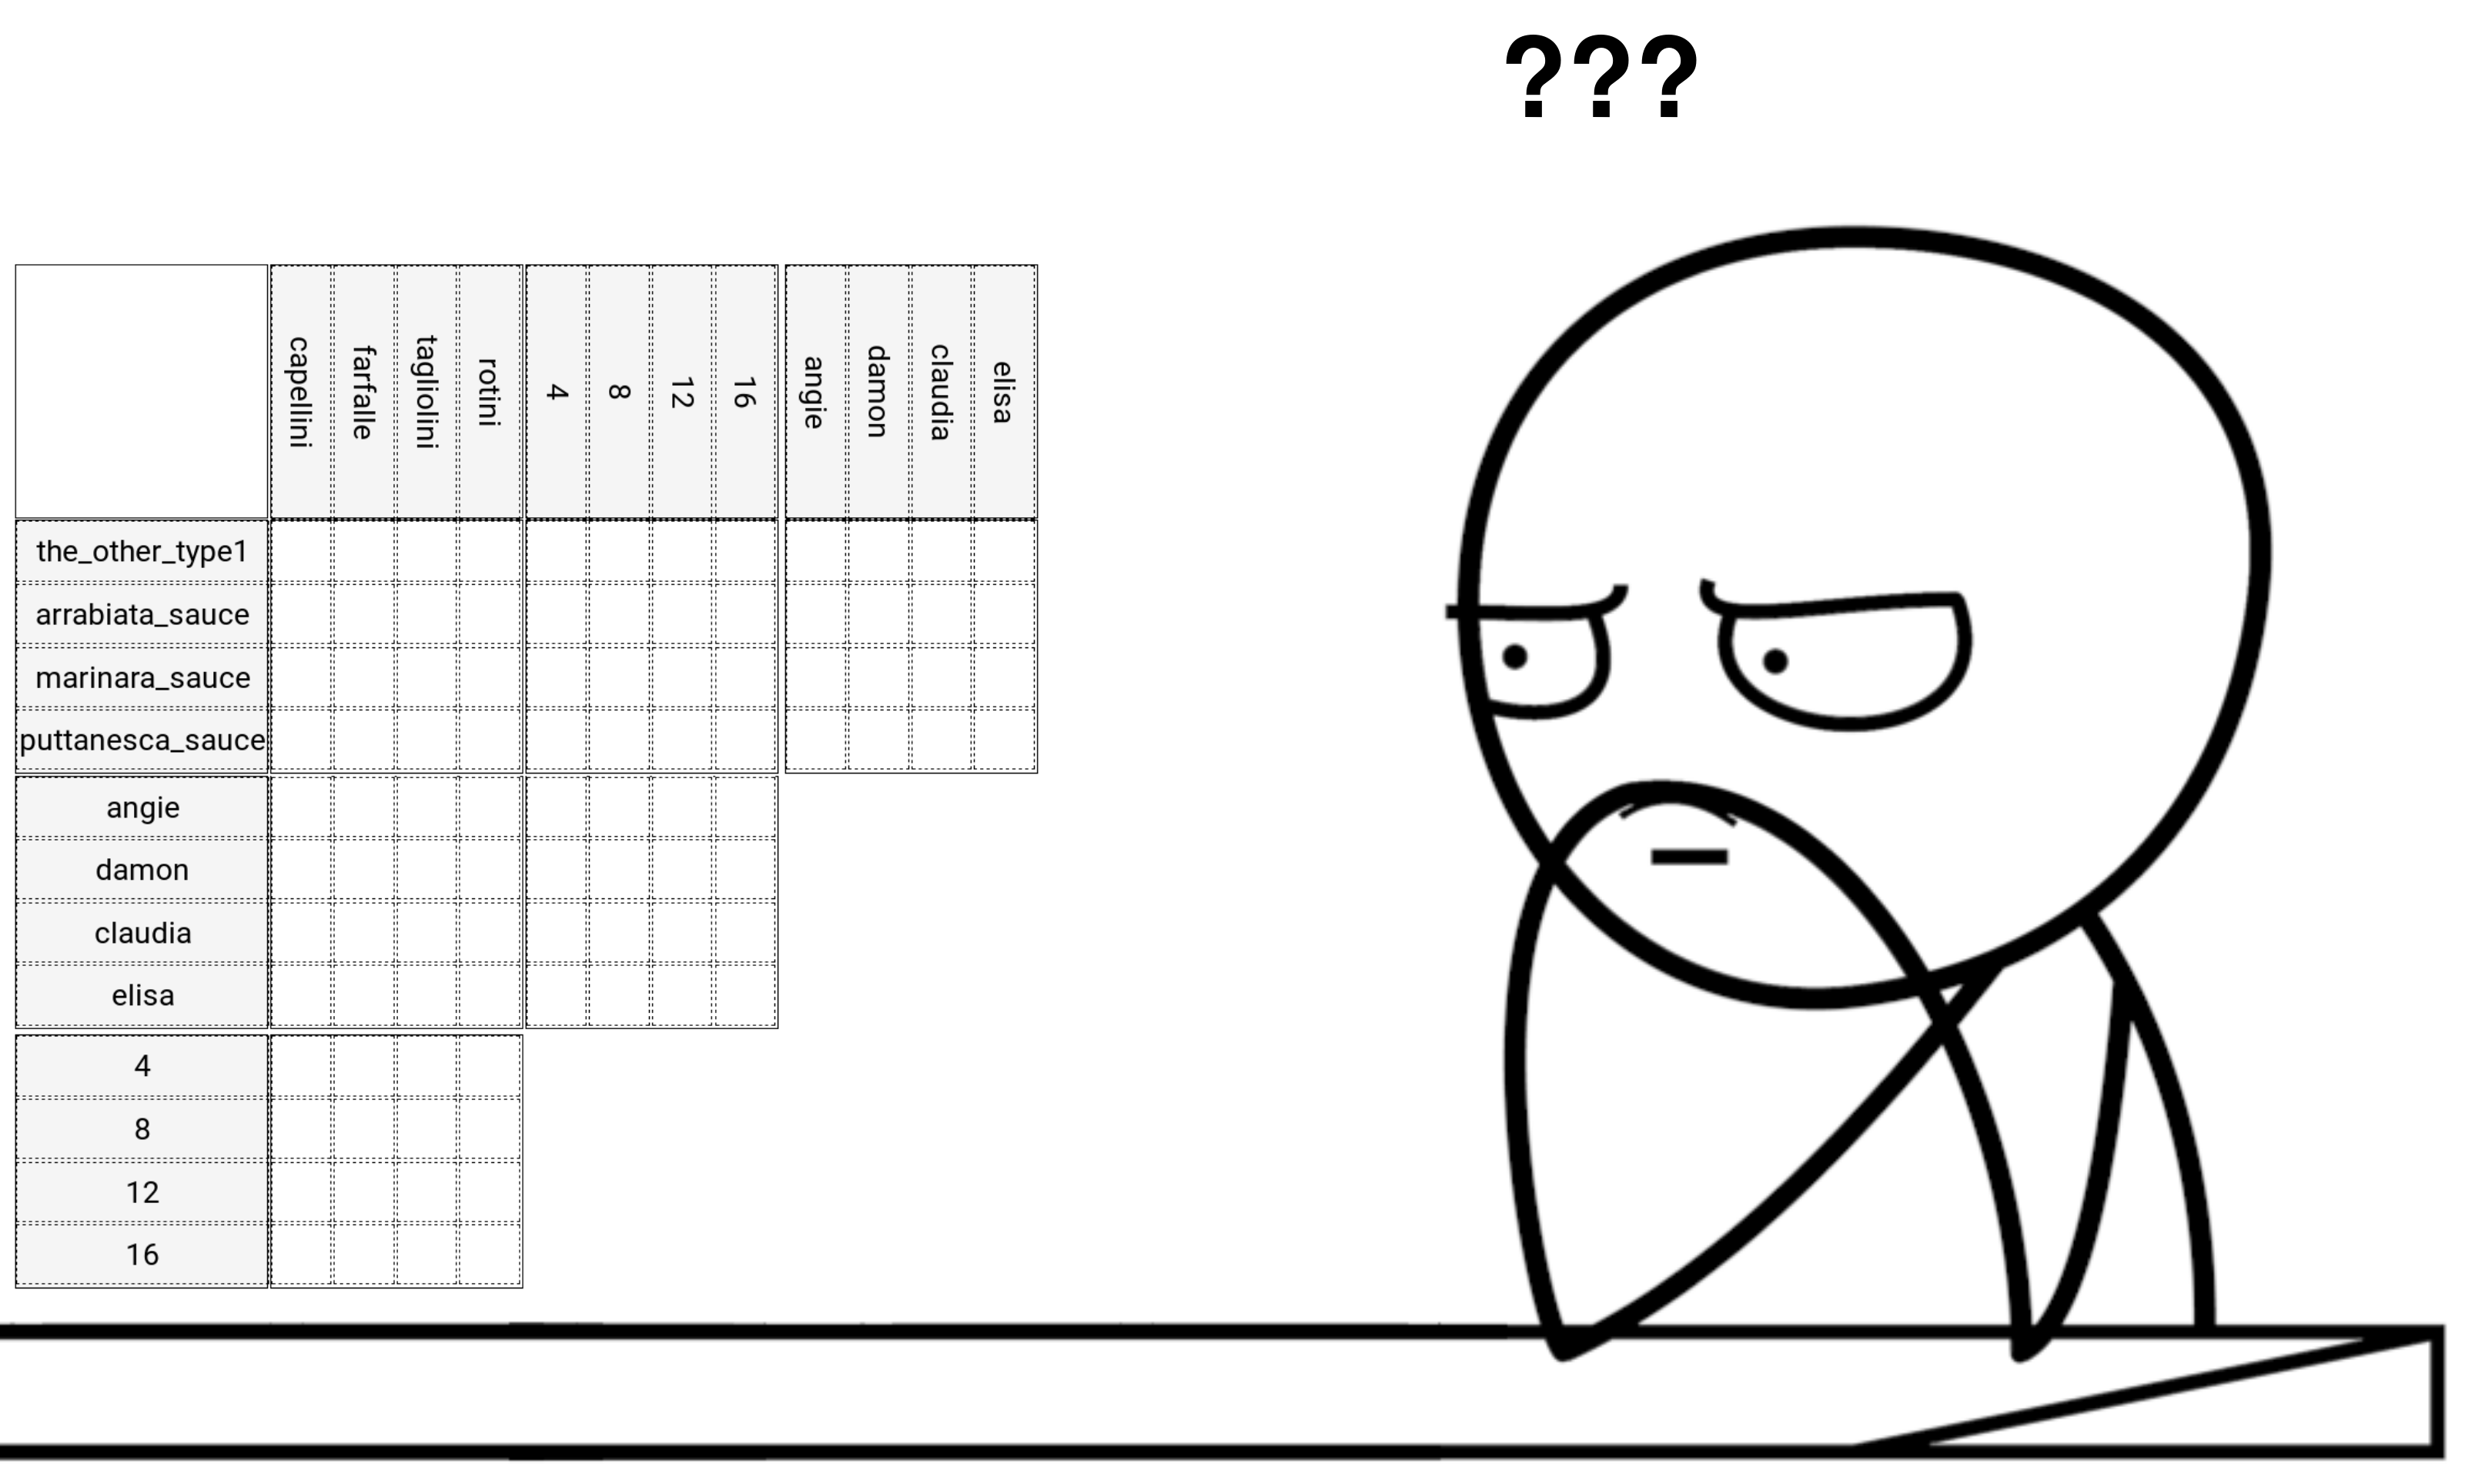
\includegraphics[width=\textwidth]{figures/meme}
            \label{grid}
        \end{figure}

    \end{minipage}
    \footnote{\tiny Figure src: \url{https://www.jing.fm/iclipt/bRTTbx/}}
\end{frame}

\begin{frame}{Motivation}
    % \framesubtitle{Motivation}
    \vfill
    % \textbf{Why constraint solving?}\pause
    \textbf{Context ?}
    \begin{itemize}
        \item \textit{Constraint solving}
              \begin{itemize}
                  \item \underline{Problem specification} is an explicit \emph{model-based representation} of the problem
                  \item Opportunity to explain inference steps in terms of this representation
              \end{itemize}
    \end{itemize}\pause
    % \textbf{Why ?}
    % \begin{itemize}
    %     \item  Our take on explainable AI with a focus on \textbf{human-interpretability}
    %           \begin{itemize}
    %               \item \emph{``Users should be able to \textbf{see} but also \textbf{study} and \textbf{understand} how inputs are (mathematically) mapped to outputs.''} \textsuperscript{\cite{doran2017does}}
    %           \end{itemize}\pause
    % \end{itemize}
    \vfill
    \textbf{How ?}
    \begin{itemize}
        \item \emph{Explain} (strong, complex) propagation in simple steps with a use case on Logic Grid Puzzles (a.k.a Zebra Puzzle, Einstein puzzle)\pause
    \end{itemize}
    \vfill
    \textbf{End-Goal ?}
    \begin{itemize}
        \item \emph{Interactive} constraint solving
    \end{itemize}

    \vfill

\end{frame}



\begin{frame}{Our Contributions}

    % \vspace{cm}
    \begin{itemize}
        \item Formalize the step-wise explanation problem;
        \item Propose an algorithm (agnostic of actual propagators, consistency level, etc.);
        \item Propose heuristics for guiding the search for explanations;
        \item Experimentally demonstrate feasibility.
    \end{itemize}
\end{frame}


\begin{frame}{Outline}

    \begin{itemize}
        \item Preliminaries
              \begin{itemize}
                  \item What is a logic grid puzzle?
              \end{itemize}
        \item Step-wise Explanations
              \begin{itemize}
                  \item Problem definition
                        \begin{itemize}
                            \item Explaining an inference step.
                            \item The explanation-production problem!
                            \item A non-redundant explanation?
                        \end{itemize}
                  \item Explanation algorithm
              \end{itemize}
              % \item 
        \item Experimental results
    \end{itemize}
    % \vfill
\end{frame}

\begin{frame}{Preliminaries}
    \begin{itemize}
        \item A logic grid puzzle instance consists of:
              \begin{itemize}
                  \item Sets of entities that need to be linked
                  \item Set of \textbf{Clues}
                  \item Each entity of one type is linked to \textit{exactly one} entity of each other type (\textbf{Bijectivity})
                  \item The links are \textit{consistent} (\textbf{Transitivity})
              \end{itemize}\pause
        \item  \textbf{Objective:}
              \begin{itemize}\small
                  \item Find the \textit{unique} assignment $I$ that satisfies all of the constraints $T$ (clues, bijectivity \& transitivity)
              \end{itemize}\pause
        \item \textit{Example}
              \begin{center}
                  \small``\textit{Angie chose arrabiate sauce and Elisa did not chose pesto}'' \\
                  % \small $I_{Ang-Ar}=\{chose(Angie,arrabiata),$ $\lnot chose(Elisa,pesto)\}$
              \end{center}
    \end{itemize}\pause

\end{frame}

\begin{frame}{Problem Definition}
    \framesubtitle{Explaining an inference step}

    \textbf{Properties}%: %of explanations for an inference step:
    \begin{itemize}
        \item Combination of {\color{vuborange}\textit{already derived facts}} \textbf{E} and {\color{vuborange}\textit{clues+constraints}} \textbf{S}
        \item \textit{\underline{Non-Redundant}}
        \begin{itemize}
            \item \textit{None} of the facts or constraints can be removed while still explaining the newly derived information
        \end{itemize}
        \item \underline{Interpretability} (difficulty) quantified by cost function $f$, ex:
              \begin{itemize}
                  \item Promote the use of simple constraints
                  \item Penalize the use of multiple constraints (combination of constraints)
              \end{itemize}
    \end{itemize}
\end{frame}

\begin{frame}{Problem Definition}
    \framesubtitle{Explanation-Production Problem}
    \textbf{Generating the explanation sequence}
    \begin{itemize}
        \item Given a \textit{theory} (clues+constraints),
        \item Starting from an \textit{initial assignment} $I_0$ (empty or partially filled grid),
        \item Find a non-redundant explanation sequence:
    \end{itemize}
    \[  I_0 \hspace{0.25cm} \xrightarrow[(E_1, S_1)]{expl.} \hspace{0.25cm} I_1 \hspace{0.25cm} \xrightarrow[(E_2, S_2)]{expl.} \hspace{0.25cm} ... \hspace{0.25cm}  \xrightarrow[(E_{n}, S_{n})]{expl.} \hspace{0.25cm} I_{n} \]
    \begin{itemize}
        \item Minimize a predefined aggregate (max, average) over the costs of the explanation sequence
    \end{itemize}

\end{frame}


\begin{frame}{Non-redundant explanation}
    \framesubtitle{...in practice}

    \begin{itemize}
        % \item \textit{Goal:} Find a non-redundant explanation
        %   \begin{itemize}
        %   \item Find a non-redundant explanation $(E \subseteq I,\ S \subseteq C, \{a\})$ that explains a new fact $a$.
        \item Smallest set of constraints and facts together explain a new fact
        \item Can be reduced to finding a Minimal Unsat Core/Subset (a.k.a MUC or MUS)
              %   , consider:
              %         \[ E\wedge S \wedge \lnot n \]
              %         \begin{itemize}
              %             \item New fact n
              %             \item $E\wedge S$ consistent
              %             \item Each unsatisfiable subset formed by $ E\wedge S \wedge \lnot n$ forms the explanation $(E ,\ S , \{a\})$
              %         \end{itemize}
              %   \end{itemize}
        \item Standard MUS extraction algorithm:
              \begin{itemize}
                %   \item If there is no satisfying solution, the unsat Core is shrunk to a Minimum Unsat Core \textsuperscript{\cite{liffiton2013enumerating}}
                  \item Subset Minimal (not further reducable), but not cardinality-minimal (the smallest one or optimal one)
              \end{itemize}
    \end{itemize}
\end{frame}

\begin{frame}{(Greedy) Algorithm}

    % {\small
    % \begin{minipage}[t]{0.58\linewidth}
    % \vfill
    \begin{itemize}
        % \item Greedy algorithm (max aggregate)
        % \begin{itemize}
            \item Generate candidate explanations using unsat-core extraction (one at a time)
            \item Iteratively grow the number of constraints used
            \item Prune search based on optimistic approximation of cost $g(C)$
        % \end{itemize}
    \end{itemize}
 
    % }
\end{frame}

\begin{frame}{(Greedy) Algorithm}
    \framesubtitle{... applied to logic grid puzzles}
    \vfill
    \begin{itemize}
        \item Visual explanation interface
        \item Cost function:
              \begin{itemize}
                  \item Single implicit axiom: very cheap
                  \item Single constraint or 1 clue: less cheap
                  \item Multiple constraints: very expensive
              \end{itemize}
    \end{itemize}
    \vfill

    \begin{center}
        \textbf{DEMO}\\
        \ \\
        \url{https://bartbog.github.io/zebra/pasta/}
    \end{center}
    \vfill
\end{frame}

\begin{frame}{Algorithm}
    \only<1>{
        \begin{minipage}[t]{0.55\textwidth}
            \centering
            \begin{figure}[]
                \centering
                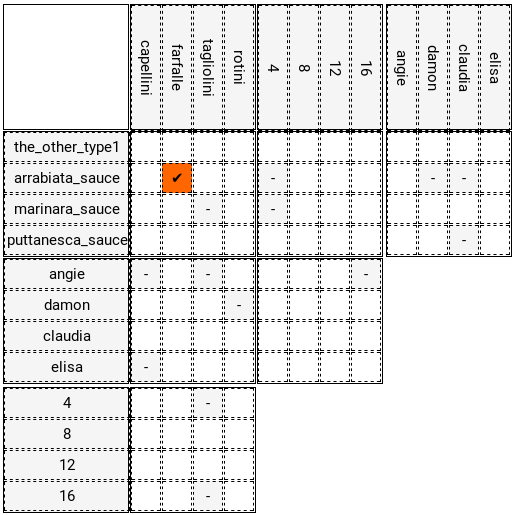
\includegraphics[width=\textwidth]{figures/step1}
                \label{step1}
            \end{figure}
        \end{minipage}\hfill
        \begin{minipage}[t]{0.40\textwidth}
            \centering
            \begin{figure}[h]
                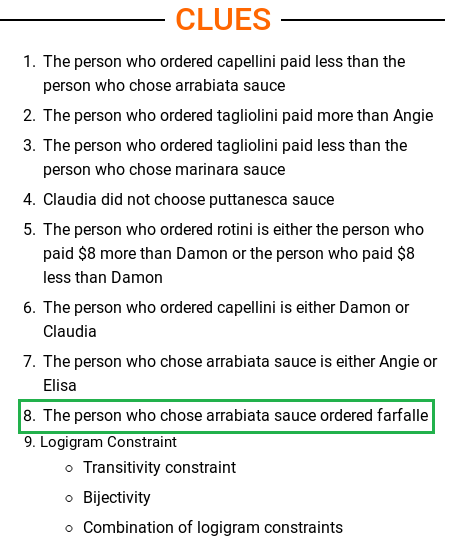
\includegraphics[width=\textwidth]{figures/clues}
                \label{clues}
            \end{figure}

        \end{minipage}

    }
    \only<2>{
        \begin{minipage}[t]{0.55\textwidth}
            \centering
            \begin{figure}[]
                \centering
                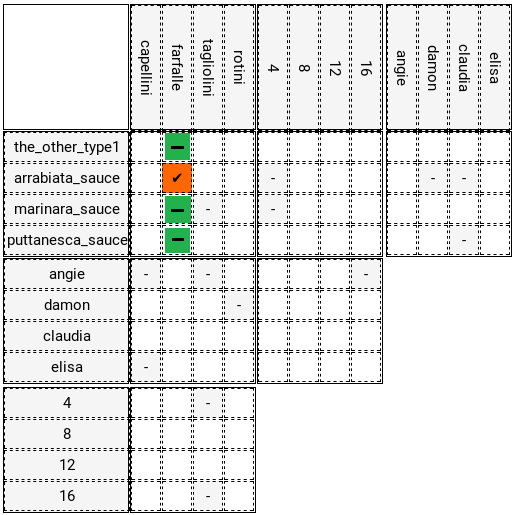
\includegraphics[height=\textwidth]{figures/possible_step1.png}
                \label{step2}
            \end{figure}
        \end{minipage}\hfill
        \begin{minipage}[t]{0.40\textwidth}
            \centering
            \begin{figure}[h]
                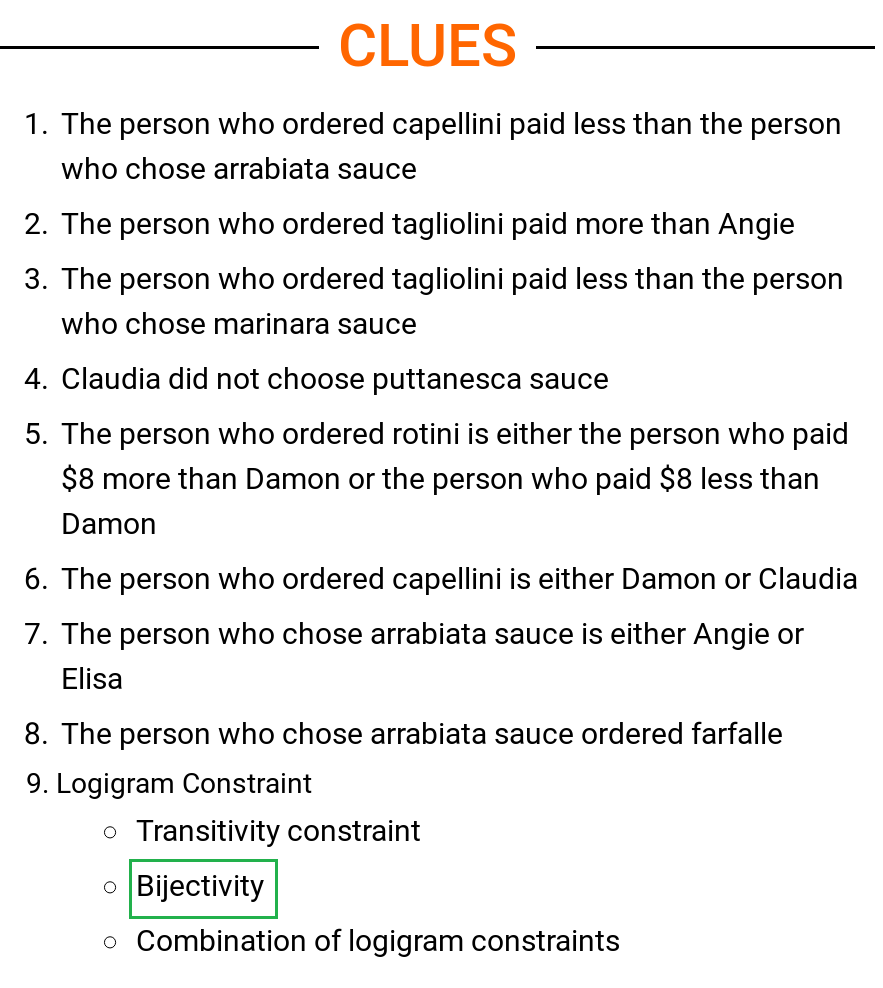
\includegraphics[width=\textwidth]{figures/clue_bijectivity.png}
                \label{clues}
            \end{figure}

        \end{minipage}

    }

    \only<3>{
        \begin{minipage}[t]{0.55\textwidth}
            \centering
            \begin{figure}[]
                \centering
                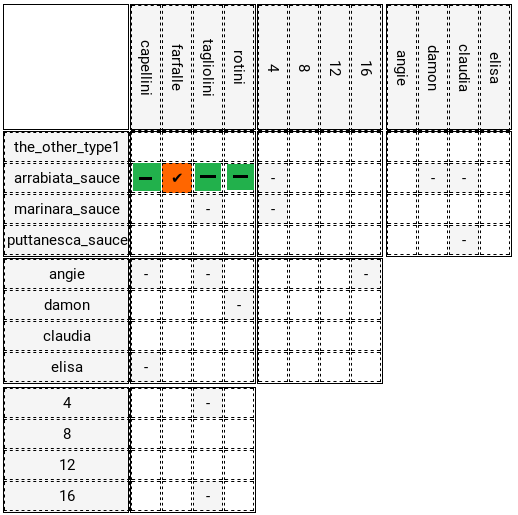
\includegraphics[height=\textwidth]{figures/possible_step2.png}
                \label{step2}
            \end{figure}
        \end{minipage}\hfill
        \begin{minipage}[t]{0.40\textwidth}
            \centering
            \begin{figure}[h]
                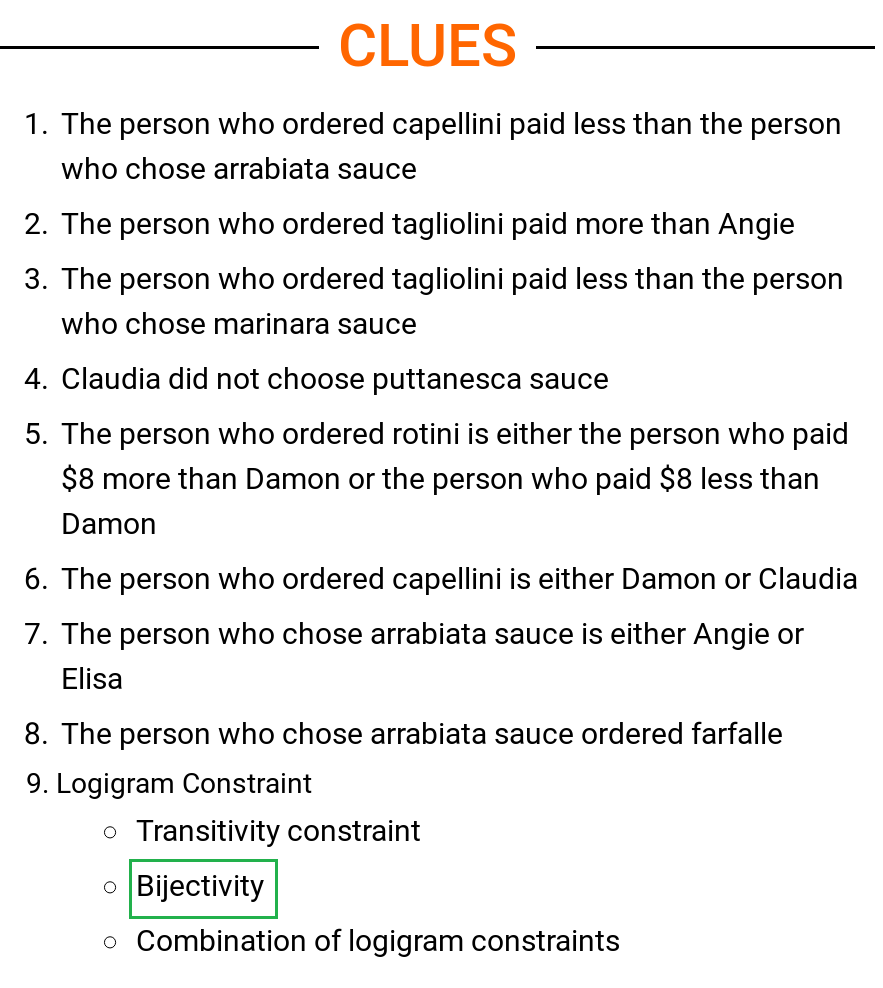
\includegraphics[width=\textwidth]{figures/clue_bijectivity.png}
                \label{clues}
            \end{figure}

        \end{minipage}

    }

    \only<4>{
        \begin{minipage}[t]{0.55\textwidth}
            \centering
            \begin{figure}[]
                \centering
                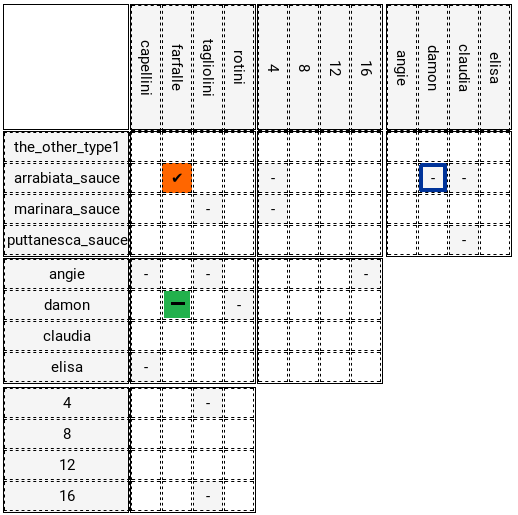
\includegraphics[height=\textwidth]{figures/possible_step3.png}
                \label{step2}
            \end{figure}
        \end{minipage}\hfill
        \begin{minipage}[t]{0.40\textwidth}
            \centering
            \begin{figure}[h]
                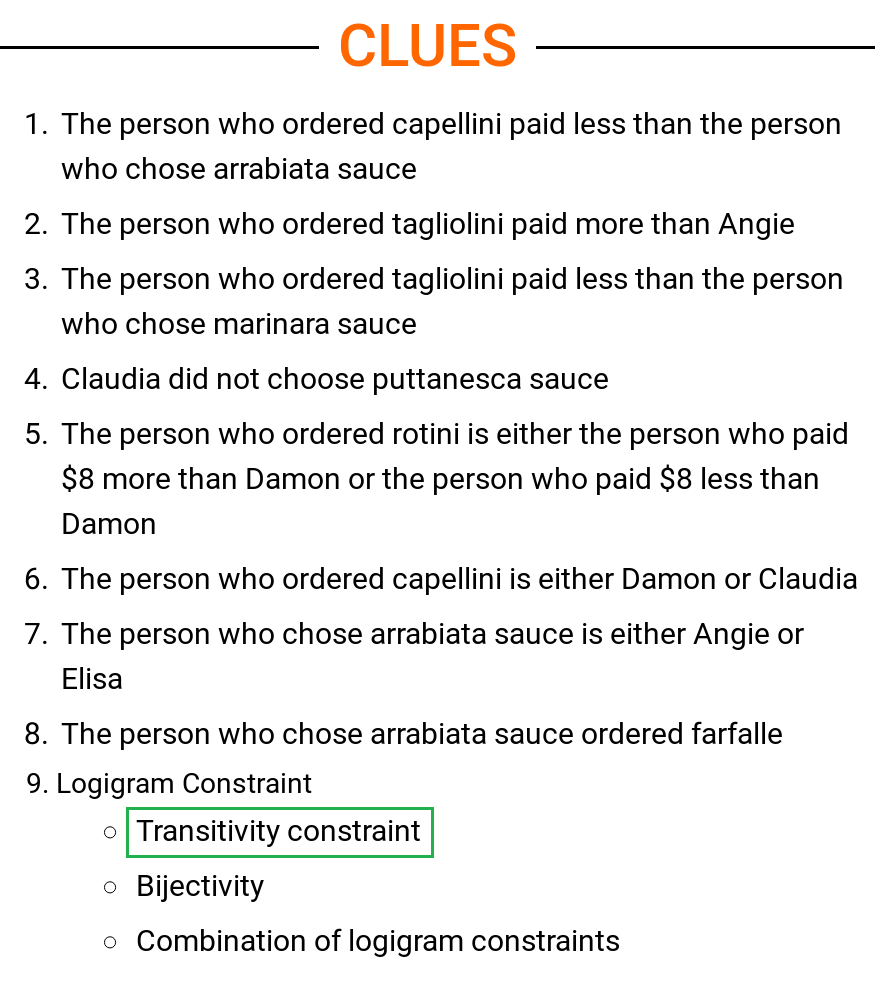
\includegraphics[width=\textwidth]{figures/clue_transitivity}
                \label{clues}
            \end{figure}

        \end{minipage}

    }

    \only<5>{
        \begin{minipage}[t]{0.55\textwidth}
            \centering
            \begin{figure}[]
                \centering
                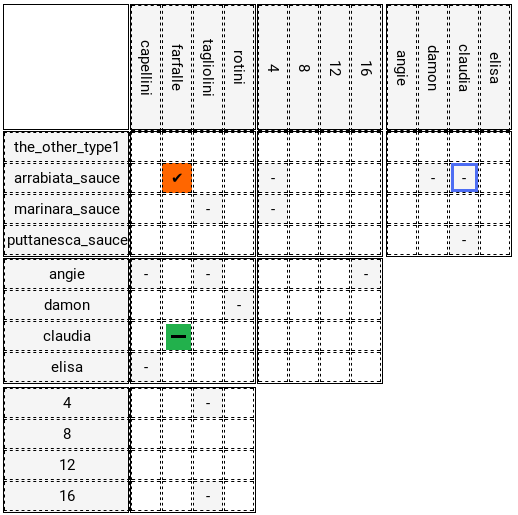
\includegraphics[height=\textwidth]{figures/possible_step4.png}
                \label{step2}
            \end{figure}
        \end{minipage}\hfill
        \begin{minipage}[t]{0.40\textwidth}
            \centering
            \begin{figure}[h]
                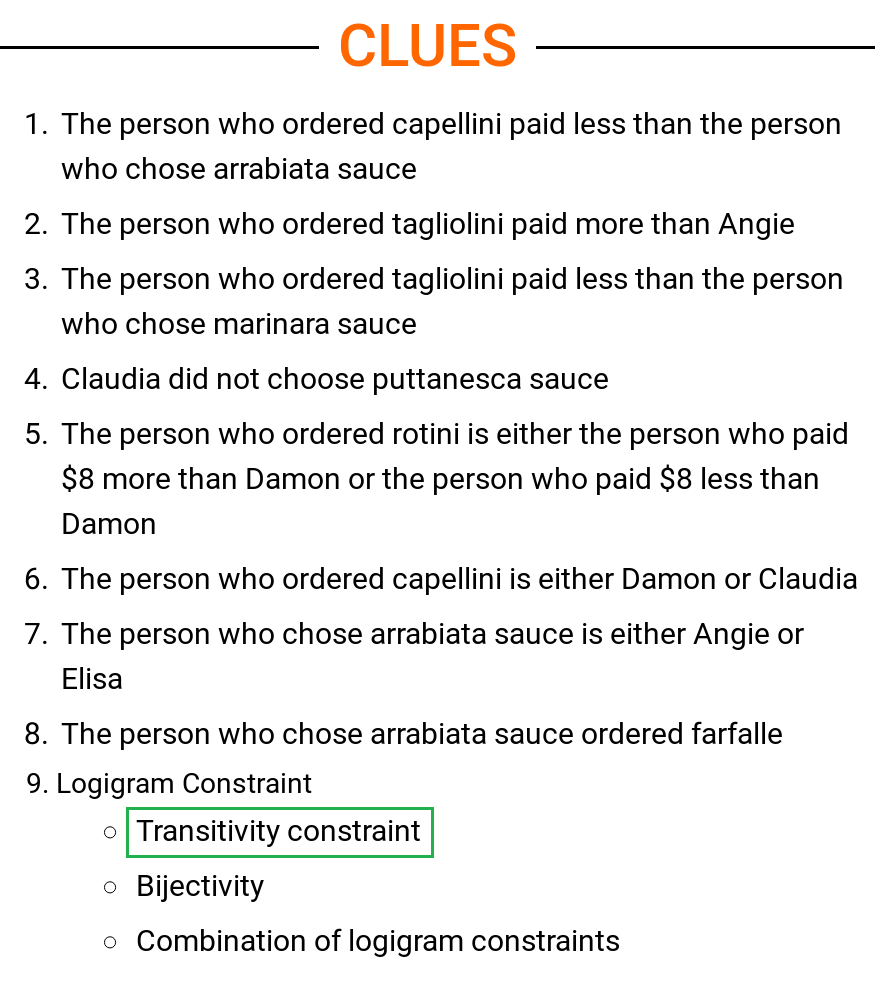
\includegraphics[width=\textwidth]{figures/clue_transitivity}
                \label{clues}
            \end{figure}

        \end{minipage}

    }

    \only<6>{
        \begin{minipage}[t]{0.55\textwidth}
            \centering
            \begin{figure}[]
                \centering
                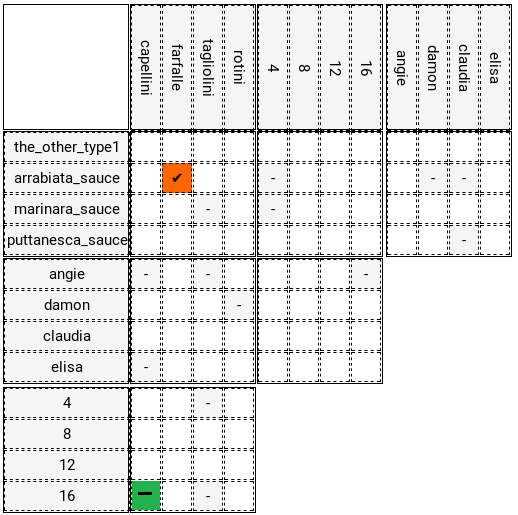
\includegraphics[height=\textwidth]{figures/possible_step5.png}
                \label{step2}
            \end{figure}
        \end{minipage}\hfill
        \begin{minipage}[t]{0.40\textwidth}
            \centering
            \begin{figure}[h]
                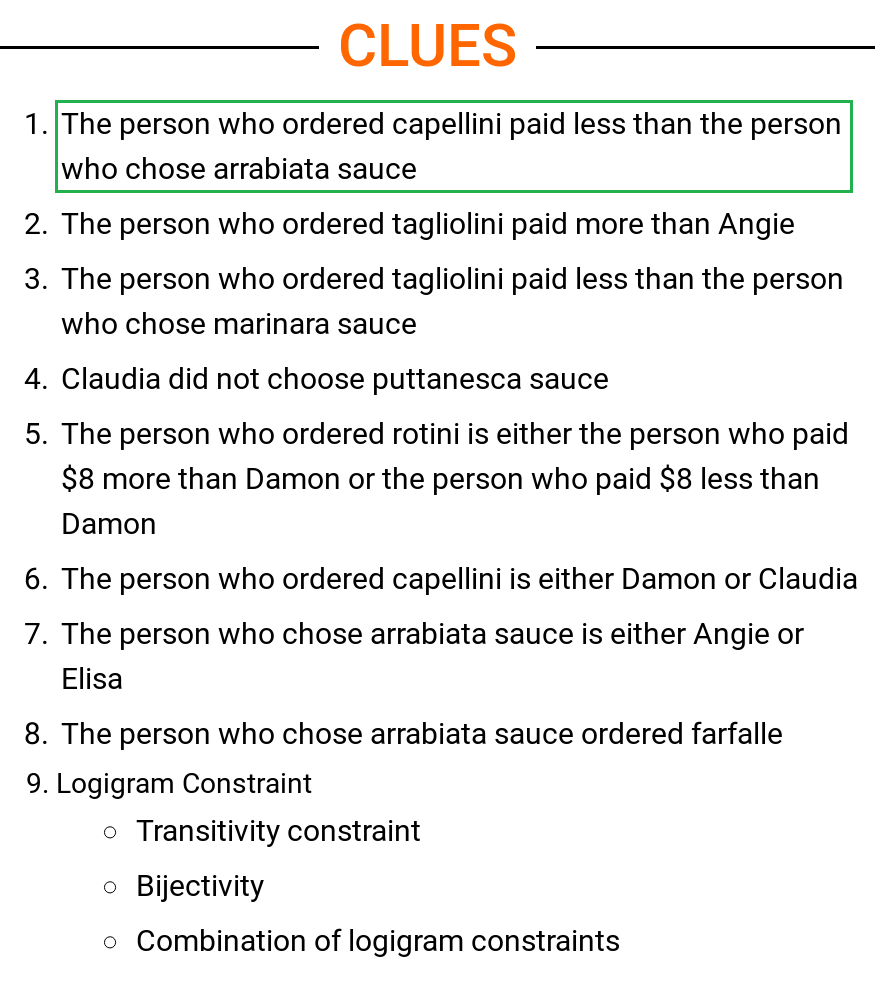
\includegraphics[width=\textwidth]{figures/clue_new_clue}
                \label{clues}
            \end{figure}

        \end{minipage}

    }



    % }
\end{frame}






\begin{frame}{Contributions}
    % \textbf{Contributions}\\
    In this paper, we
    \begin{itemize}
        \item ... formalize the \emph{step-wise explanation problem},
        \item ... propose a greedy algorithm (agnostic of actual propagators, consistency level, etc.),
        \item ... propose heuristics for \emph{guiding} and \emph{speeding-up the search for \underline{easy-to-understand} explanations},
        \item ... use logic grid puzzle to show the feasibility of the approach.
    \end{itemize}
\end{frame}

\begin{frame}{Use cases}
    \begin{itemize}
        \item Teach humans how to solve a certain problem
        \item Quantify problem difficulty
        \item ``Help'' button
        \item Interactive configuration/planning/scheduling
    \end{itemize}
\end{frame}

\begin{frame}{Conclusion and Future work}

    \textbf{Current work}
    \begin{itemize}
        \item Extension to support nested explanations \textsuperscript{\cite{bogaerts2020framework}}
        \item Optimal explanations for inference step using unsat-core optimization \textsuperscript{\cite{ignatiev2013quantified}}
    \end{itemize}\pause
    \vfill
    \textbf{Future work}
    \begin{itemize}
        \item Optimize the explanation sequence
        \item Learning the optimization function (from humans)
        \item Interactive configuration \textsuperscript{\cite{fox2017explainable, van2017kb, carbonnelle2019interactive}}
    \end{itemize}
    \vfill
\end{frame}



% \bibliographystyle{abbrv}
\bibliographystyle{plainnat}
\begin{frame}{References}
    % \frametitle
    % \vspace{2em}
    \tiny \bibliography{references}
\end{frame}

\end{document}



\begin{frame}{What about the explanation sequence?}

    \begin{figure}
        \centering
        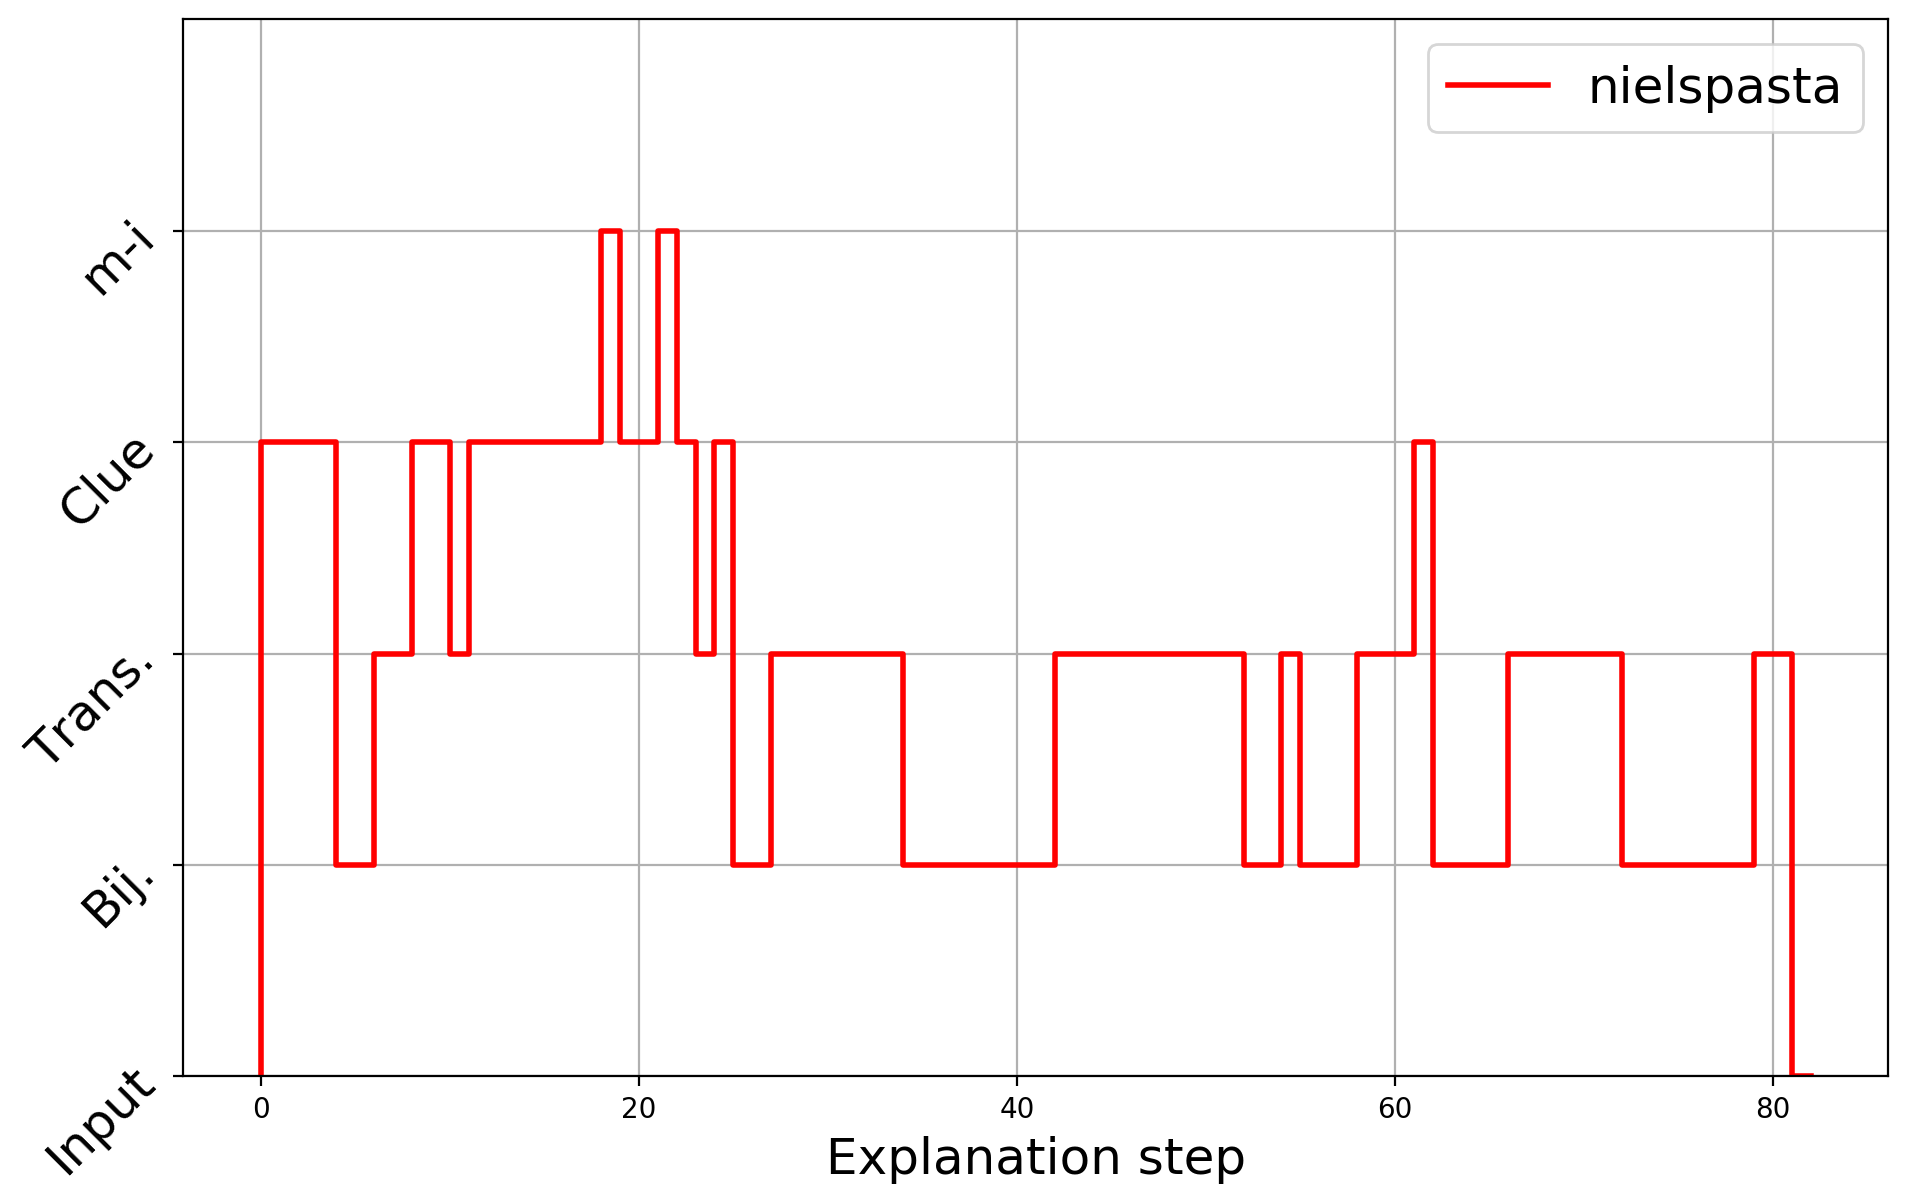
\includegraphics[width=0.6\textwidth]{plot_cost_steps_nielspasta}
        \label{pasta-puzzle}
        \caption{Type of constraints used in each step}
    \end{figure}

\end{frame}
% \begin{frame}{Problem Definition}
%     \framesubtitle{Explaining an inference step}
%     % \begin{definition}
%     % \begin{itemize}
%     % {\small
%     % \item 
%     Let $I_{i-1}$ and $I_i$ be partial interpretations such that $I_{i-1}\wedge T \models I_i$.
%     We say that {\color{vuborange}$(E_i,S_i,N_i)$ \emph{explains} the derivation of $I_{i}$ from $I_{i-1}$} if the following hold:\pause
%     \begin{itemize}
%         \item $N_i= I_i \setminus I_{i-1}$ (i.e., $N_i$ consists of all newly defined facts), \pause
%         \item $E_i\subseteq I_i$ (i.e., the explaining facts are a subset of what was previously derived),\pause
%         \item $S_i \subseteq T_P$ (i.e., a subset of the clues and implicit constraints are used), and \pause
%         \item $S_i \cup E_i \models N_i$ (i.e., all newly derived information indeed follows from this explanation).
%     \end{itemize}

%     % \end{itemize}
%     %     \pause

%     %     \begin{figure}[]
%     %         \centering
%     %         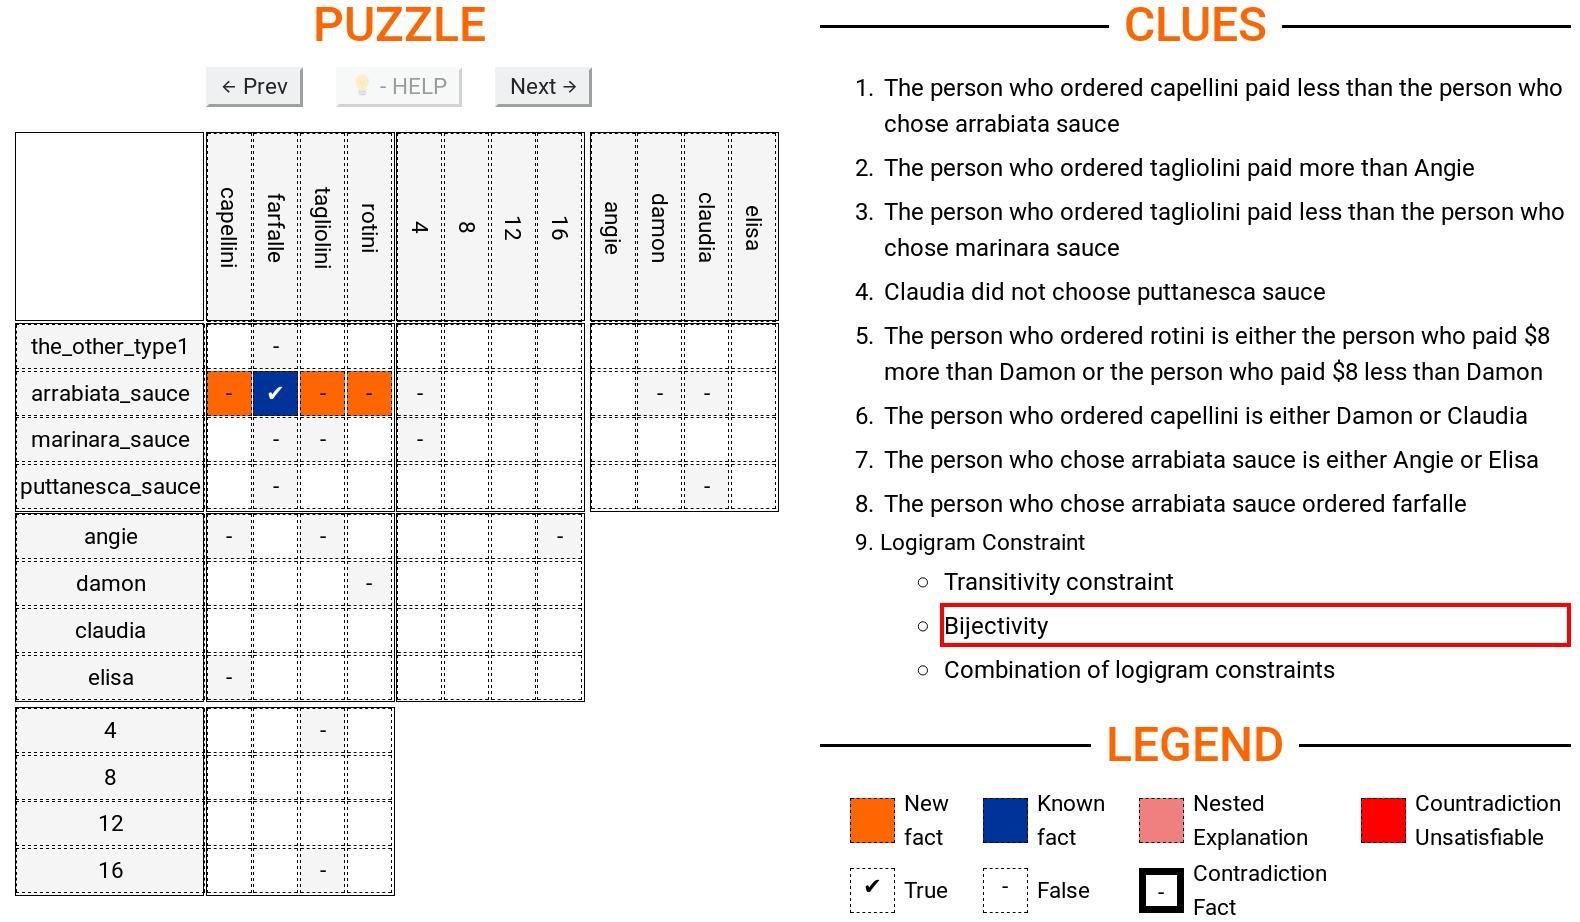
\includegraphics[width=0.6\textwidth]{figures/introduction.jpeg}
%     %         \label{lapin}
%     %     \end{figure}
%     % % \end{definition}
% \end{frame}

% \begin{frame}{Problem Definition}
%     \framesubtitle{A non-redundant (easy) explanation}
%     \begin{definition}
%         We call $(E_i,S_i,N_i)$ a {\color{vuborange}\emph{non-redundant explanation of  the derivation of $I_i$ from $I_{i-1}$}} if it explains this derivation and whenever $E'\subseteq E_i; S'\subseteq S_i$ while $(E',S',N_i)$ also explains this derivation, it must be that $E_i=E', S_i=S'$.
%     \end{definition}
%     \pause
%     Furthermore, we assume existence of a \emph{cost function} $f(E_i,S_i,N_i)$ that quantifies the interpretability of a single explanation.

% \end{frame}

% \begin{frame}{Problem Definition}
%     \framesubtitle{Quantifying explanation difficulty}

%     \textbf{Example}
%     \begin{align*}   & f(E,S) = basecost(S) + |E| + |S|                              \\
%          & g(S) = basecost(S) = \left\{\begin{array}{ll}
%             0             & \text{if $|S|=1$ and $nc(S) = 0$} \\
%             20            & \text{if $|S|>1$ and $nc(S)=0$}   \\
%             20\cdot nc(S) & \text{otherwise}
%         \end{array}\right.
%     \end{align*}    \textit{Interpretation:}
%     \begin{itemize}
%         \item Penalize the use of multiple constraints (combination of constraints)
%         \item Promote the use of simple constraints
%     \end{itemize}

% \end{frame}

% \begin{frame}{Problem}
%     \framesubtitle{Generating the explanation sequence}
%     \begin{definition}
%         Given a theory $T$ and initial partial interpretation $I_0$, the {\color{vuborange}\emph{explanation-production problem}} consist of finding a non-redundent explanation sequence
%         \[(I_0,(\emptyset,\emptyset,\emptyset)), (I_1,(E_1,S_1,N_i)), \dots ,(I_n,(E_n,S_n,N_n))\]
%         such that a predefined aggregate over the sequence $\left(f(E_i,S_i,N_i)\right)_{i\leq n}$ is minimised.
%     \end{definition}
% \end{frame}

% \begin{frame}{Explainable Artificial Intelligence (XAI)}
%     \framesubtitle{Curse of performance vs Interpretability}
%     \vfill
%     \textbf{Curse of performance}
%     \begin{itemize}
%         \item Black-box prediction systems (e.g. deep neural networks)
%         \item Efficient complex reasoning systems with millions of parameters
%     \end{itemize}
%     \vfill
%     \pause
%     \textbf{Need for Explainable AI (XAI)} \textsuperscript{\cite{gunning2017explainable, miller2019explanation}}
%     \begin{itemize}
%         \item Verify correctness of the system
%         \item Control for unbiased or unfair decisions \pause
%         \item \textbf{Predictions systems} (ML)\textsuperscript{\cite{adadi2018peeking}}:
%               \begin{itemize}
%                   \item Justify why certain predictions are made ;
%                   \item What part of the input is important in the \textit{learned} model? \textsuperscript{\cite{samek2017explainable}}
%               \end{itemize}\pause
%         \item \textbf{Constraint solving}
%               \begin{itemize}
%                   \item Understand the inference steps required for computing the solution
%                   \item Explain overconstrained, unsatisfiable problems to a user
%               \end{itemize}
%     \end{itemize}
%     % \pause
%     % \textbf{The A.R.T of Responsible AI (Adadi et al, 2018)\textsuperscript{\cite{adadi2018peeking}}}\pause
%     % \begin{itemize}
%     %     \item \textbf{\underline{A}ccountability} \textit{need to explain and justify actions to user}
%     %     \item \textbf{\underline{R}esponsibility} \textit{role of answering for one's decisions and identify errors or unexpected results}
%     %     \item \textbf{\underline{T}ransparency} \textit{need to describe, inspect and reproduce AI thought process}
%     % \end{itemize}
%     \vfill
% \end{frame}

% \begin{frame}{Still difficult steps...}

%     \begin{figure}
%         \centering
%         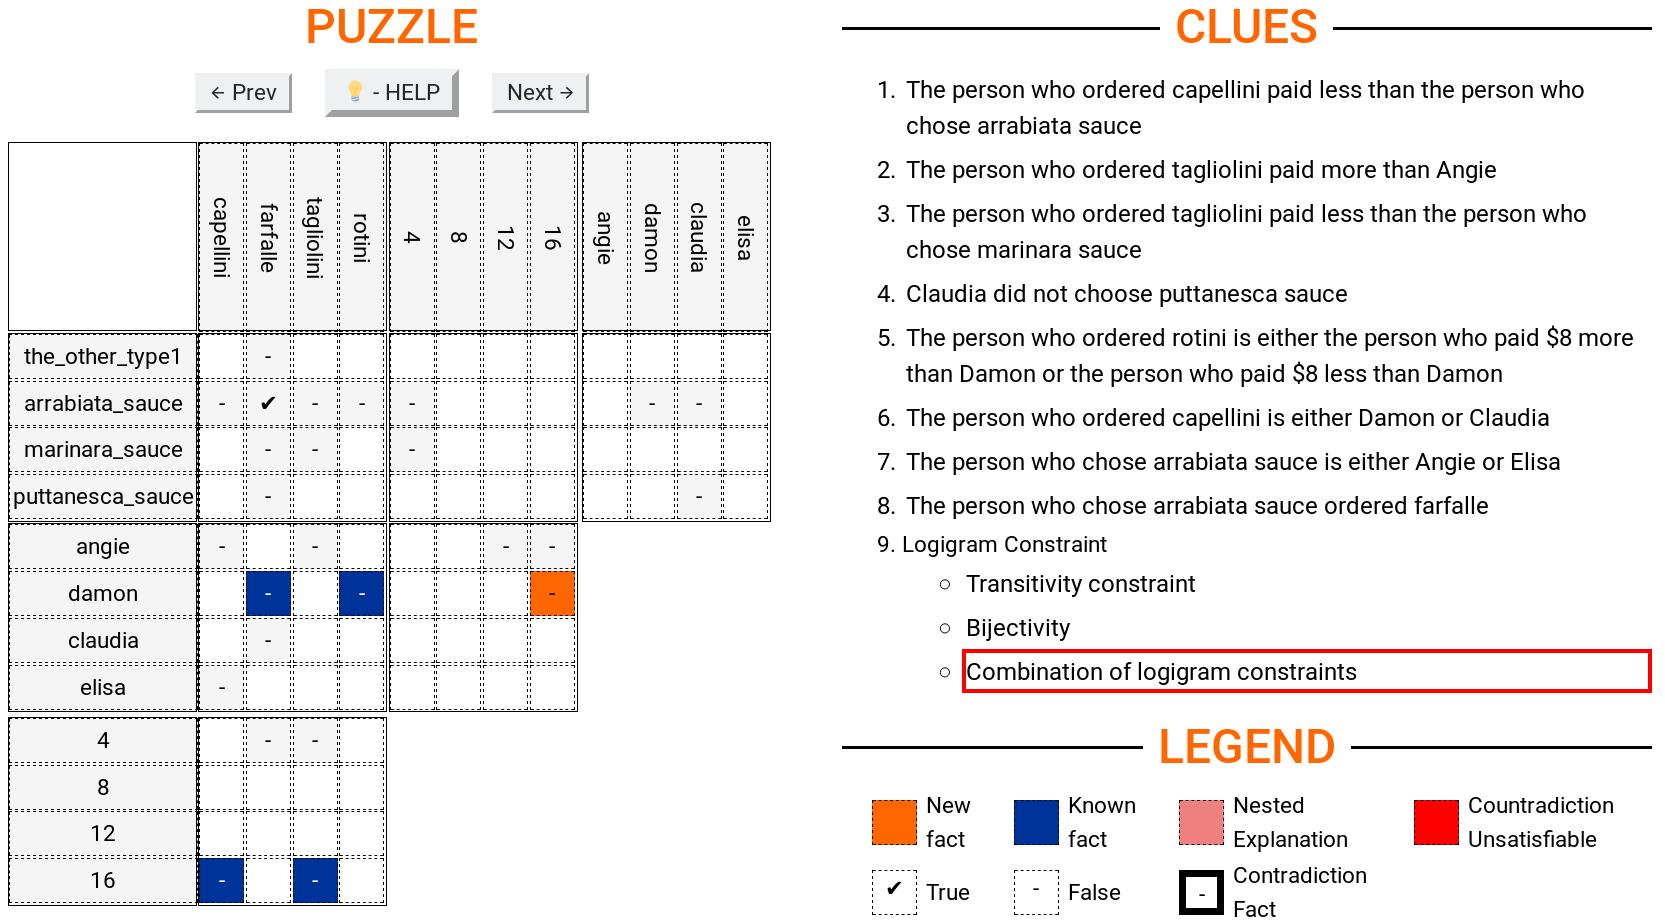
\includegraphics[width=\textwidth]{figures/related_work.jpeg}
%         \label{pasta-puzzle2}
%         % \caption{Example of a difficult step}
%     \end{figure}

% \end{frame}


